\subsubsection{Functional Requirements}
\begin{itemize}
  \item The system shall know the time when an User do a reservation.
  \item The system shall tag a car avaible again if a car is not picked-up within an hour from the reservation.
  \item The system shall apply a fee of 1 EUR if a car is not picked-up within an hour from the reservation.
\end{itemize}

\subsubsection{Scenario 1}
Mark needs to go to the city center in the late evening and decides to use a PowerEnJoy's car. Just before having a quick lunch in a near restaurant he browses the application and reserves car near him to make sure that it will still be available when he'll be back.
Unexpectedly Morgan, a friend of Mark, is lunching in the same restaurant and when they see each other they start chatting about everything and anything. When they stop talking Mark notices an e-mail from PowerEnJoy: it's about his reservation that has expired. His bank has also notified him that a fee of 1€ was applied by PowerEnJoy.

%\subsubsection{Mockups}
%\begin{figure}[!ht]
%  \centering
% \vspace{0.1cm}
% 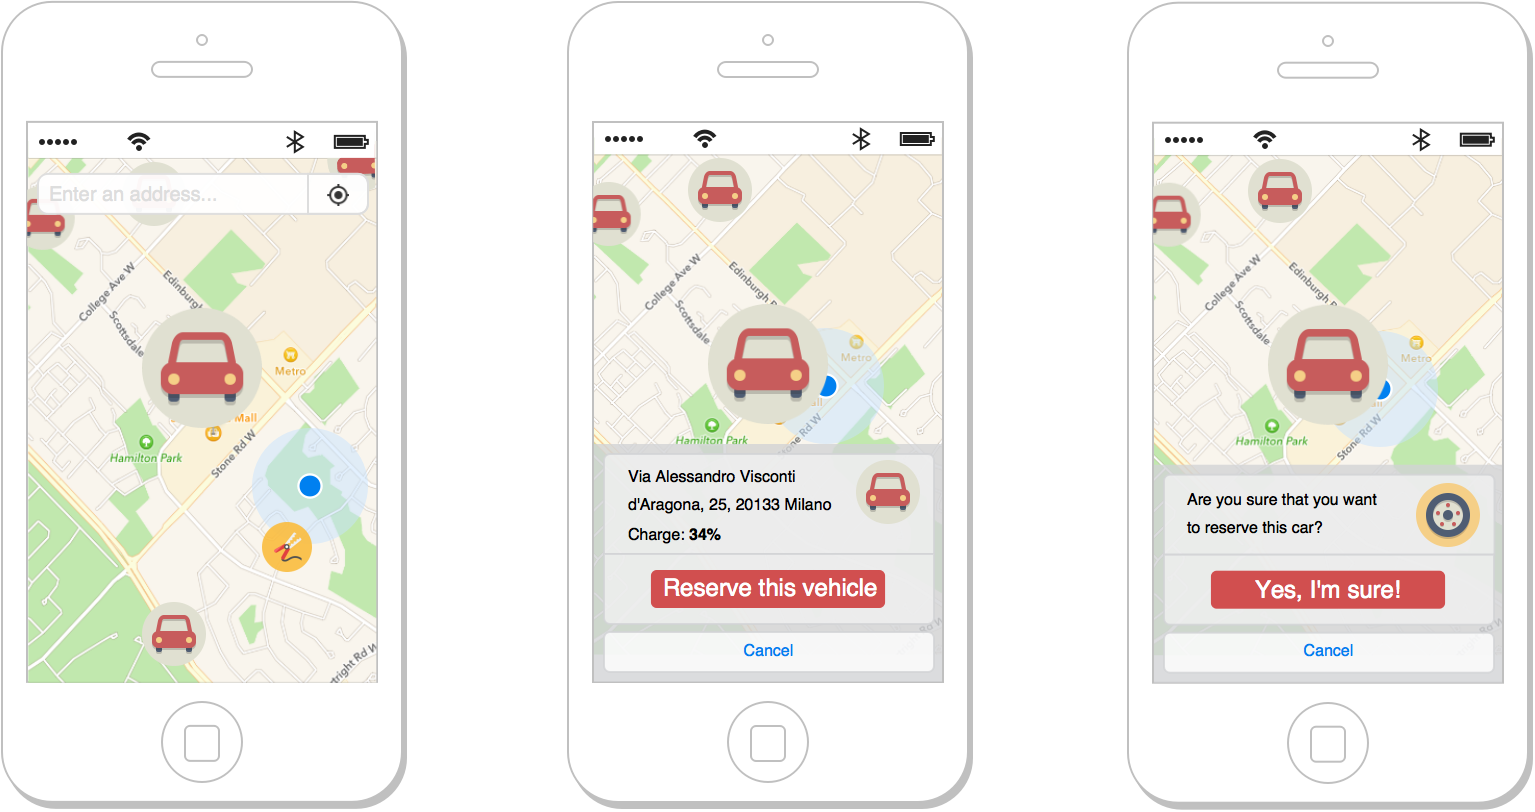
\includegraphics[width=1\textwidth]{/RASD/System_Functions/create_reservation_mockup}\\
%  \vspace{0.4cm}
%  %\caption{Mockup for the login mobile page} 
% \label{fig:create_reservation_mockup} 
%\end{figure}
% maybe home page mockup here 


\subsubsection{Use-case table}
\begin{center}
  \begin{tabular}{ l | p{10cm} }
    \hline
    Actors & User\\ \hline
    Goal & G\ref{itm:goal-reservation}\\ \hline
    Entry conditions & \begin{itemize}
			\item The User has reserved a car.
			\item The system has activeted the timer.
\end{itemize}  \\ \hline
    Flow of events &
\begin{itemize}
\item The system checks the timer. If it's up an hour the reservetion is expired.
\item The system applies a fee of 1€ to the User.
\item The system notified the User.
\item The User pays the fee.
\item The system notifies the User of the success of the payment.
\item The system turn the car "available".
\end{itemize} \\ \hline
    Exit conditions &
\begin{itemize}
	\item A car is set as "available".
	\item The User's reservation is delated.
\end{itemize}  \\ \hline
  Exceptions & 
\begin{itemize}
\item The timer has some issues.
\item The payment failed.
\item The system is not able to complete the operation due to some internal issues or connection broken (the system signals a ConnectionFailure).%volendo si possono modificare i nomi delle eccezzioni.
\end{itemize} 
\\ \hline
  \end{tabular}
\end{center}


\newpage
\subsubsection{Sequence diagram}
\begin{figure}[!ht]
  \centering
  \vspace{0.2cm}
  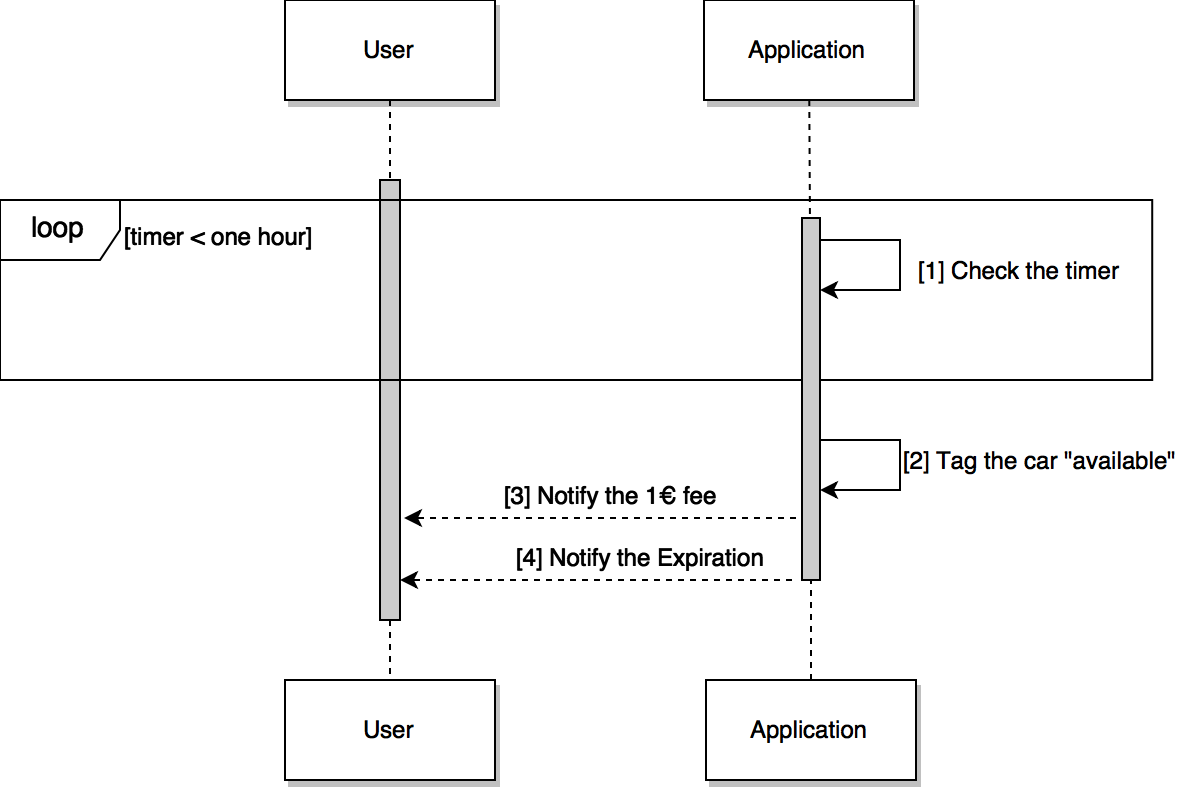
\includegraphics[width=0.8\textwidth]{/RASD/System_Functions/expirationofthereservation_sequence}\\
  \vspace{0.1cm}
  %\caption{Sequence diagram for the login procedure} 
  \label{fig:expirationofthereservation_sequence} 
\end{figure}

